\section{System Description}
\begin{frame}{System Description}
	\subsection{System Overview}
	\framesubtitle{System Overview}
	\begin{figure}[H]
		\centering
		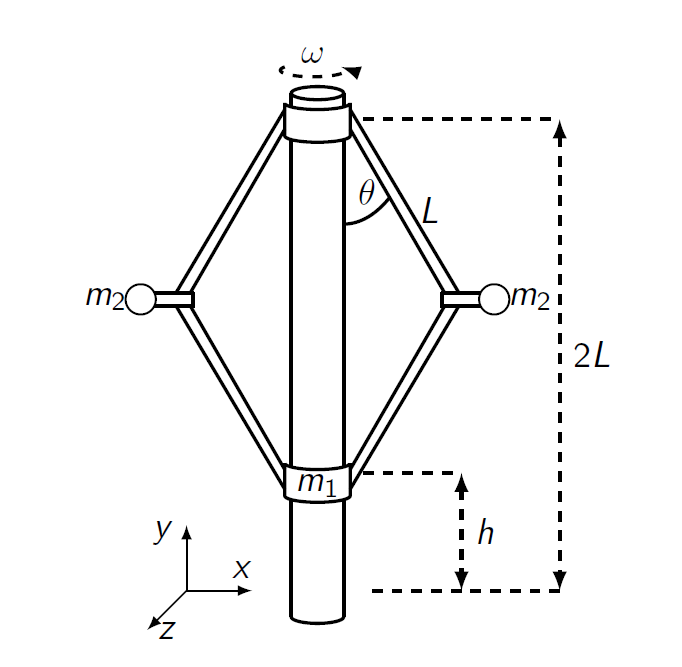
\includegraphics[width=0.80\textwidth]{pics/overview.png}
	\end{figure}
\end{frame}

\subsection{Position Vectors}
\begin{frame}{System Description}
	\framesubtitle{Position Vectors}
	\begin{equation*}
	\vv{r}_{m2,1} = \left(\begin{array}{c}
	L\sin(\theta)\cos(\beta)\\ L(2-\cos(\theta)) \\ -L\sin(\theta)\sin(\beta)
	\end{array}\right)
	\end{equation*}
	\begin{equation*}
	\vv{r}_{m2,2} = \left(\begin{array}{c}
	-L\sin(\theta)\cos(\beta)\\ L(2-\cos(\theta)) \\ L\sin(\theta)\sin(\beta)
	\end{array}\right)
	\end{equation*}
	\begin{equation*}
	\vv{r}_{m1} = \left(\begin{array}{c}
	0\\ 2L(1-\cos(\theta)) \\ 0
	\end{array}\right)
	\end{equation*}
	\centering mit $\beta = \int \omega dt$
\end{frame}